\documentclass[12pt]{article}
\usepackage{epsf}
\usepackage{amssymb}
\usepackage{enumitem}
\usepackage{amsmath}
\usepackage{tikz}

\title{aashlock-331-hw0}
\author{Aren Ashlock}
\date{January 23, 2024}

\setlength{\oddsidemargin}{-0.25in}
\setlength{\topmargin}{-0.5in}
\setlength{\headheight}{0cm}
\setlength{\headsep}{0cm}
\setlength{\textheight}{10in}
\setlength{\textwidth}{7in}
\setlength{\topskip}{0cm}

\begin{document}

\noindent\textbf{ComS 331 \quad Spring 2024 \quad Name: Aren Ashlock}

\begin{enumerate}

%----------------------------------- Q1 DONE -----------------------------------

\item Reproduce the text and figure...

\fbox{\parbox{\textwidth}{
This is an inline equation: $x + y = 3$.

This is a displayed equation:
\begin{displaymath}
    x + \frac{y}{z - \sqrt{3}} = 2
\end{displaymath}

This is how you can define a piece-wise linear function:
\begin{displaymath}
    f(x) = \begin{cases}
        {3x} + 2 & \mbox{if $x < 0$}\\
        {7x} + 2 & \mbox{if $x \geq 0$ and $x < 10$}\\
        {5x} + 22 & \mbox{otherwise}\\
    \end{cases}
\end{displaymath}

This is a matrix:
\begin{displaymath}
    \begin{array}{|c|c|c|c|} \hline
        9 & 9 & 9 & 9 \\ \hline
        6 & 6 & 6 & \\ \hline
        3 & & 3 & 3 \\ \hline
    \end{array}
\end{displaymath}

This is a graph with two types (solid and dashed) of labeled edges:
\begin{center}
    \begin{tikzpicture}
        \node[draw=black, fill=lightgray, circle] (p) at (0,0) {$p$};
        \node[draw=black, fill=lightgray, circle] (r) at (1.75, 0.75) {$r$};
        \node[draw=black, fill=lightgray, circle] (q) at (1.75, -0.75) {$q$};

        \path [->, dashed] (p) edge node[near start, below] {$t_1$} (q);
        \path [->, dashed, bend right = 10] (q) edge node[midway, right] {$t_2$} (r);
        \path [->] (r) edge node[near start, below] {$t_3$} (p);
    \end{tikzpicture}
\end{center}
}}

%-------------------------------------------------------------------------------

%----------------------------------- Q2 DONE -----------------------------------

\item Prove that $\mathbb{N}$ (natural numbers) and $\mathbb{Z}$ (integer numbers) are equinumerous.

We can prove that two sets are equinumerous through the existence of a bijection.\\
First, we must define a function $f(n)$ that maps the values of one set to another.\\
$f(n) = \begin{cases}
    - \frac{n}{2} & \mbox{if n is even}\\
    \frac{n + 1}{2} & \mbox{if n is odd}
\end{cases}$\\
\textbf{One-to-one:} $\forall a, b \in \mathbb{N}, f(a) = f(b) \implies a = b$\\
\textit{N is even:} $-\frac{a}{2} = -\frac{b}{2} \rightarrow a = b$\\
\textit{N is odd:} $\frac{a + 1}{2} = \frac{b + 1}{2} \rightarrow a = b$\\
\textbf{Onto:} $\forall a, b \in \mathbb{N}, f(a) = f(b) \implies a = b$\\
\textit{N is even:} $f(a) = b \rightarrow -\frac{a}{2} = b \rightarrow a = -2b$\\
\textit{N is odd:} $f(a) = b \rightarrow \frac{a + 1}{2} = b \rightarrow a = 2b - 1$\\
\textbf{Since,} the function is both one-to-one and onto, this proves that there is a bijection between $\mathbb{N}$ and $\mathbb{Z}$. This means that they are equinumerous.

%-------------------------------------------------------------------------------

%----------------------------------- Q3 DONE -----------------------------------

\item Prove that the relation $R$ defined by $\forall m, n \in \mathbb{N}, (m, n) \in R \Leftrightarrow (m - n) \text{ mod } 3 = 0$ is an equivalence relation, and describe its equivalence classes.

We prove this by showing that the relation is reflexive, symmetric, and transitive.\\
\textbf{Reflexive:} $\forall x \in \mathbb{N}, (x, x) \in R$:\\
$(x - x) \text{ mod } 3 = 0 \text{ mod } 3 = 0$\\
\textbf{Symmetric:} $\forall x, y \in \mathbb{N}, (x, y) \in R \implies (y, x) \in R$:\\
$(x - y) \text{ mod } 3 = 0 \rightarrow x - y = 3k$\\
$(y - x) = 3(-k) \text{: } 3(-k) \text{ mod } 3 = 0$\\
$\therefore (y, x) \in R$\\
\textbf{Transitive:} $\forall x, y, z \in \mathbb{N}, (x, y) \in R \wedge (y, z) \in R \implies (x, z) \in R$:\\
$(x - y) \text{ mod } 3 = 0 \wedge (y - z) \text{ mod } 3 = 0$\\
$(x - y + y - z) \text{ mod } 3 = 0$\\
$(x - z) \text{ mod } 3 = 0$\\
\textbf{Since,} the relation $R$ is reflexive, symmetric, and transitive, that means it IS an equivalence relation.\\
\textbf{Equivalence Classes:}\\
$[0]_R = \{3k | k \in \mathbb{N}\}$\\
$[1]_R = \{1 + 3k | k \in \mathbb{N}\}$\\
$[2]_R = \{2 + 3k | k \in \mathbb{N}\}$

%-------------------------------------------------------------------------------

%----------------------------------- Q4 DONE -----------------------------------

\item Show that $\sum^{n}_{i=1} i^2 = (2n + 1)(n + 1)n/6$

We prove this by using induction on n.\\
\textbf{Basis:} This holds for $n = 0$, since $\sum^0_{i=1} i^2 = 0$ and $(2(0) + 1)(0 + 1)0/6 = 0$.\\
\textbf{Induction Hypothesis:} Assume that $\forall m \leq n$, $\sum^m_{i=1} i^2 = (2m + 1)(m + 1)m/6$.\\
\textbf{Inductive Step:} Then, the property holds for $n + 1$ as well, since...\\
$\sum^{n+1}_{i=1} i^2 = (2(n + 1) + 1)((n + 1) + 1)(n + 1)/6$\\
$\sum^n_{i=1} i^2 + (n + 1)^2 = (2(n + 1) + 1)((n + 1) + 1)(n + 1)/6$\\
$(2n + 1)(n + 1)n/6 + n^2 + 2n + 1 = (2(n + 1) + 1)((n + 1) + 1)(n + 1)/6$\\
$(2n^3 + 3n^2 + n)/6 + (6n^2 + 12n + 6)/6 = (2(n + 1) + 1)((n + 1) + 1)(n + 1)/6$\\
$(2n^3 + 9n^2 + 13n + 6)/6 = (2(n + 1) + 1)((n + 1) + 1)(n + 1)/6$\\
$(2(n + 1) + 1)((n + 1) + 1)(n + 1)/6 = (2(n + 1) + 1)((n + 1) + 1)(n + 1)/6$\\
The equality above is \textbf{TRUE}. Therefore, $\sum^{n}_{i=1} i^2 = (2n + 1)(n + 1)n/6$.

%-------------------------------------------------------------------------------

%----------------------------------- Q5 DONE -----------------------------------

\item Show that, for $n \geq 1$, $\sum\limits^{n}_{i=1}\frac{1}{i^2} \leq 2 - \frac{1}{n}$.

We prove this by using induction on n.\\
\textbf{Basis:} This holds for $n = 1$, since $\sum\limits^{1}_{i=1}\frac{1}{i^2} = 1$ and $2 - \frac{1}{1} = 1$ and $1 \leq 1$.\\
\textbf{Induction Hypothesis:} Assume that $\forall m \leq n$, $\sum\limits^{m}_{i=1}\frac{1}{i^2} \leq 2 - \frac{1}{m}$ when $m \geq 1$.\\
\textbf{Inductive Step:} Then, the property holds for $n + 1$ as well, since...\\
$\sum\limits^{n + 1}_{i=1}\frac{1}{i^2} \leq 2 - \frac{1}{n + 1}$\\
$\sum\limits^n_{i=1}\frac{1}{i^2} + \frac{1}{(n + 1)^2} \leq 2 - \frac{1}{n + 1}$\\
$2 - \frac{1}{n} + \frac{1}{(n + 1)^2} \leq 2 - \frac{1}{n + 1}$\\
$- \frac{1}{n} + \frac{1}{(n + 1)^2} \leq - \frac{1}{n + 1}$\\
$- \frac{(n + 1)^2}{n(n + 1)^2} + \frac{n}{n(n + 1)^2} \leq - \frac{n(n + 1)}{n(n + 1)^2}$\\
$\frac{n - n^2 - 2n - 1}{n(n + 1)^2} \leq \frac{-n^2 - n}{n(n + 1)^2}$\\
$\frac{-n^2 - n - 1}{n(n + 1)^2} \leq \frac{-n^2 - n}{n(n + 1)^2}$\\
The equality above is \textbf{TRUE}. Therefore, for $n \geq 1$, $\sum\limits^{n}_{i=1}\frac{1}{i^2} \leq 2 - \frac{1}{n}$.

%-------------------------------------------------------------------------------

\end{enumerate}
\end{document}